\begin{figure}
  \centering
  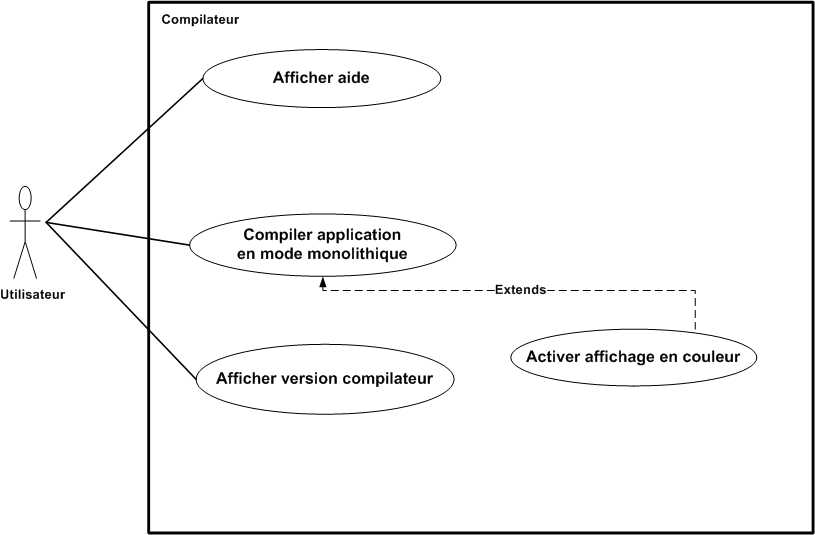
\includegraphics[scale=0.5]{../res/stb/UseCase_AfterChange.png}
  \caption{\textbf{Cas d'utilisations du compilateur kawa.}}
\end{figure}

%Cas d'utilisation
\subsection{Cas d'utilisation EF\_1}
\fiche
{Afficher l'aide}                    % Nom du cas d'utilisation
{Utilisateur du compilateur}                               % Acteurs concernés
{                                                % Description
  le compilateur affiche 
   la liste des options du compilateur sur la sortie standard à travers une ligne de commande.
}
{
  L'ordre de priorité entre le commutateur de help (-h ou -\hspace{0.1mm}-help) et le commutateur de version (-v ou -\hspace{0.1mm}-version) est définit par le commutateur en premier paramètre. Le commutateur -h/-\hspace{0.1mm}-help est le premier paramètre obligatoirement.
}                                                % Préconditions
{Commutateur de ligne de commande :kawac -h ou -\hspace{0.1mm}-help }                             % Evénements déclenchants
{L'aide a été affichée correctement et la main est redonnée à l'utilisateur pour entrer d'autres commutateurs.}                       % Conditions d'arrêt
% {0.6}{../res/stb/usecase2_flot_event.png}      % Diagramme
{} % acteur(s)
{} % system
{} % flot exceptionsb
 % fin usecase EF_1

\subsection{Cas d'utilisation EF\_2}
\fiche
{Compiler une application en mode monolithique}                    % Nom du cas d'utilisation
{Utilisateur du compilateur}                               % Acteurs concernés
{                                                % Description
  L'utilisateur introduit un ensemble de modules (classe/interface)
  kawa afin de les précompiler et de générer une application sous forme d'un seul exécutable.
}
{
	Afin de permettre la compilation dans ce mode monolithique il faut:
	\begin{itemize}
  	\item Indiquer l’emplacement des fichiers sources de l'application.
  	\item Introduire le commutateur  \textbf {-m}  en premier paramètre dans la ligne de commande permettant la compilation.
  	\item L'absence des deux commutateurs (-h ou -\hspace{0.1mm}-help) et (-v ou -\hspace{0.1mm}-version) en premier paramètre.
  	\end {itemize}
}                                                % Préconditions
{

Afin de pouvoir lancer la compilation dans ce mode l'utilisateur  doit: 
\begin{itemize}
  	\item Indiquer au moins un module (une classe avec une méthode main qui constitue le point d'entrée d'une application).
  	\item Introduire une ligne de commande avec un commutateur d'action: kawac -m filessources.
 \end {itemize}

}    % Evénements déclenchants
{
	\begin{itemize}
  	\item La compilation s'est terminée sans erreurs dans ces différentes étapes d’analyses.
  	\item La production d’un unique fichier exécutable sous le format d'ELF  qui ne dépend d'aucune bibliothèque kawa ainsi que le nom du fichier exécutable correspond au nom du module contenant la méthode main.
\end {itemize}
  
}  % Conditions d'arrêt
%{0.6}{../res/stb/usecase2_flot_event.png} 		 % Diagramme
{                                                % Flots d'exceptions
  
}
{} % system
{
La compilation peut être interrompue pour divers raisons, on cite:

	\begin{itemize}
  	\item \textbf {EF\_2\_EXC\_1}: Le fichier de sortie n'a pu être créé.
  	\item  \textbf {EF\_2\_EXC\_2}: Le code source d'un des modules de l'application comporte une erreur syntaxique, l'erreur rencontrée pendant cette étape d'analyse est renvoyée sur la sortie standard du compilateur.
  	\item \textbf {EF\_2\_EXC\_3}: Le code source d'un des modules (classe/interface) dont dépend le programme est introuvable. Un message renvoyé par le compilateur indique le nom du (ou des) module(s) manquants sur la sortie standard.
  	\item \textbf {EF\_2\_EXC\_4}: Le code source d'un des modules de l'application comporte une erreur sémantique, exemple : l'incompatibilité de type statique lors d'une opération d'affectation.
  	\item \textbf {EF\_2\_EXC\_5}: Aucun des modules indiqués ne comporte le point d'entrée (main).
  	\item \textbf {EF\_2\_EXC\_6}: Plusieurs méthodes main ont été trouvées parmi les classes indiquées dans le source, le compilateur renvoie la liste des points d'entrée trouvés sur la sortie standard.
  	\end {itemize}
 } % flot exceptions
% Fin de la fiche du cas d'utilisation 1.


%Cas d'utilisation 2

% Fin de la fiche du cas d'utilisation 2.


%Cas d'utilisation

% Fin de la fiche du cas d'utilisation 3.
%Cas d'utilisation
\subsection{Cas d'utilisation EF\_3}
\fiche
{Afficher la version du compilateur}                      % Nom du cas d'utilisation
{Utilisateur du compilateur}                               % Acteurs concernés
{                                                % Description
   
L'utilisateur peut savoir la version du compilateur avec le quel compile ses sources et ses bibliothèques  à travers un commutateur de ligne de commande.   
}
{
   L'odre de priorité entre le commutateur de help (-h ou -\hspace{0.1mm}-help) et le commutateur de version (-v ou -\hspace{0.1mm}-version) est définit par la première occurrence de l'un des deux commutateur i-e si nous avons un \textbf {-v} avant un \textbf {-h}, le compilateur annule tout le reste et affiche la version
}                                                % Préconditions
{Commutateur de ligne de commande:kawac -v ou -\hspace{0.1mm}-version}                             % Evénements déclenchants
{La version est affichée sur la sortie standard du compilateur.}                       % Conditions d'arrêt
%{0.6}{../res/stb/usecase3_flot_event.png}     % Diagramme
{                                                % Flots d'exceptions
 
}{} % system
{} % flot exceptions
% Fin de la fiche du cas d'utilisation 3.

% Fin de la fiche du cas d'utilisation 3.

%Cas d'utilisation
\subsection{Cas d'utilisation EF\_4}
\fiche
{Activer l'affichage en couleur}          % Nom du cas d'utilisation
{Utilisateur du compilateur}                               % Acteurs concernés
{                                                % Description
   
  L'utilisateur peut activer l'option de l'affichage en couleur, afin de décorer les messages renvoyés par le compilateur la sortie standard dans les différents modes de compilation.   
}
{
  
}                                                % Préconditions
{Commutateur de ligne de commande:kawac filessource -\hspace{0.1mm}-color}  % Evénements déclenchants (--help) \verb+kawac -h ou --help+ -----> pour creer u espace entre --
{Le code présent sur la sortie standard a été colorié.}                       % Conditions d'arrêt
%{0.6}{../res/stb/usecase3_flot_event.png}     % Diagramme
{                                                % Flots d'exceptions
 
}{} % system
{} % flot exceptions
% Fin de la fiche du cas d'utilisation 3.